\documentclass{article}
\usepackage[utf8]{inputenc}
\usepackage[T1]{fontenc}
\usepackage[french]{babel}
\usepackage{lmodern}
\usepackage{amsmath}
\usepackage{amssymb}
\usepackage{pgf,tikz}
\usepackage{graphicx}
	
\title{Analyse de sentiments}
\author{Frédéric \textsc{Wantiez} -- Pierre \textsc{Vigier}}

\begin{document}

\maketitle

\section{Description du problème}

\subsection{Intérêt}

\subsection{Formalisation}

L'analyse de sentiments est un problème d'apprentissage supervisé. Notons $V$ l'ensemble de tous les mots possibles et $V^{*}=\cup_{n \geq 0}{V^{n}}$ l'ensemble des textes sur ce vocabulaire. Soit $x_{1}, ..., x_{N} \in V^{*}$ des textes et $y_{1}, ..., y_{N} \in S$ le sentiment associé à chacun des textes. Ces sentiments peuvent être des valeurs dans $S=[0, 1]$ où $0$ signifie que le texte est "très négatif" et $1$, "très positif". Une variante plus simple est d'avoir les $(y_{i})_{i \in {1, ..., N}}$ dans $S={0, 1}$ où 0 signifie "négatif" et $1$, "positif". Notre objectif est de déterminer une fonction $f$ telle que $\forall i \in {1, ..., N}, y_{i} \approx f(x_{i})$ et qui devra, de plus, bien généraliser sur des textes jamais vus auparavant. Dans le cas où $S$ est discret, il s'agit d'un problème de classification. Dans le cas continu, il s'agit d'un problème de régression.

Nous allons essentiellement nous concentrer sur le problème de classification. Plusieurs types d'entrée et plusieurs types de classifieurs seront essayés sur le problème. La mesure de performance choisie est la précision $A(y_{1}, ..., y_{N}, \hat{y}_{1}, ..., \hat{y}_{N}) = \frac{\sum_{i=0}^{N}{1_{y_{i}=\hat{y}_{i}}}}{N}$. L'objectif est de la maximiser. Elle nous permettra de comparer les performances des différents algorithmes.

\section{Données}

Il est assez facile de créer un ensemble de données pour entraîner nos algorithmes. En effet, il suffit de trouver un site où l'on peut commenter et mettre des notes sur des produits. La valeur numérique de la note correspond alors au sentiment dégagé par le texte. Cette configuration est présente sur les sites d'e-commerce comme Amazon ou sur les sites de critiques comme IMDB ou Rotten Potatoes.

% Comment on détermine le sentiment sur les tweets ?

Nous utilisons l'ensemble de données mis à disposition par Maas et al. \cite{maas-EtAl:2011:ACL-HLT2011}. Il s'agit d'un ensemble de 50 000 avis en anglais sur IMDB. Il est découpé en un ensemble d'apprentissage et un ensemble de test. À chaque avis est associé un label $0$ ou $1$ selon que l'avis est positif ou négatif. Le label $0$ correspond à une note inférieure à $4$ tandis que le label $1$ correspond à une note supérieure à $7$. Les notes de $5$ et $6$ sont exclues car représentant un avis neutre. Il y a autant d'avis positifs que d'avis négatifs dans l'ensemble d'apprentissage ainsi que dans l'ensemble de test. Dans la figure \ref{example_imdb}, on retrouve un avis négatif et un avis positif. On remarque que des fragments de code HTML et des libertés typographiques peuvent être présents.

\begin{figure}[h]
\begin{center}
\begin{tabular}{|c|c|p{80mm}|}
	\hline
	id & sentiment & review \\
	\hline
	\texttt{0\_3} & \texttt{0} & \texttt{Story of a man who has unnatural feelings for a pig. Starts out with a opening scene that is a terrific example of absurd comedy. A formal orchestra audience is turned into an insane, violent mob by the crazy chantings of it's singers. Unfortunately it stays absurd the WHOLE time with no general narrative eventually making it just too off putting. Even those from the era should be turned off. The cryptic dialogue would make Shakespeare seem easy to a third grader. On a technical level it's better than you might think with some good cinematography by future great Vilmos Zsigmond. Future stars Sally Kirkland and Frederic Forrest can be seen briefly.} \\
	\hline
	\texttt{9999\_8} & \texttt{1} & \texttt{The plot had some wretched, unbelievable twists. However, the chemistry between Mel Brooks and Leslie Ann Warren was excellent. The insight that she comes to, ""There are just moments,"" provides a philosophical handle by which anyone could pick up, and embrace, life.<br /><br />That was one of several moments that were wonderfully memorable.} \\
	\hline
\end{tabular}
\caption{Exemple d'un commentaire négatif et d'un commentaire positif extrait de l'ensemble d'apprentissage.}
\label{example_imdb}
\end{center}
\end{figure}

\subsection{Méthodologie}

Afin de mener notre étude, nous avons choisi d'utiliser le langage Python (version 3.5) qui a l'avantage de présenter un écosystème de technologies liées à l'apprentissage automatique qui est développé et accessible. Nous utiliserons notamment les libraires suivantes :
\begin{itemize}
	\item \textit{pandas} pour manipuler et analyser des données ;
	\item \textit{Numpy} pour l'algèbre linéaire ; 
	\item \textit{Matplotlib} pour les graphiques ;
	\item \textit{scikit-learn} pour les algorithmes d'apprentissage automatique ;
	\item \textit{TensorFlow} pour les réseaux de neurones ;
	\item \textit{NLTK} pour manipuler le langage naturel.
\end{itemize}

Nous allons devoir faire face à plusieurs difficultés. Premièrement, nous devons prétraiter les avis en enlevant le code HTML. Nous devrons aussi réussir à modéliser les avis, qui sont des chaînes de caractères de taille variable, par des caractéristiques permettant d'utiliser des algorithmes d'apprentissage. La plupart d'entre eux nécessitant des entrées de taille fixe et numériques. Finalement, nous verrons que réussir à modéliser l'ordre des mots sera une nécessité pour atteindre améliorer la précision de la classification.

Notre démarche est assez simple, nous allons procéder par complexité croissante. Nous allons commencer par utiliser les modèles et algorithmes les plus "naïfs" puis analyser faiblesses de chaque  méthode afin d'avancer et proposer des solutions pour améliorer nos résultats.

\section{Premières tentatives}

Nous allons commencer par utiliser deux représentations pour nos textes, la première étant les sacs de mots et la seconde se basant sur les vecteurs de mot. Dans chaque cas, nous allons nous concentrer sur la création des caractéristiques. Nous utiliserons pour commencer des algorithmes d'apprentissage relativement simples.

\subsection{Sac de mots}

\subsubsection{Description}

Les sacs de mots \cite{Salton:1986:IMI:576628} est une représentation très simple. Numérotons les éléments de $V$, on a alors $V={w_{1}, ..., w_{D}}$. Prenons un texte $t \in V^{*}$ et notons $tf_{i,t} = card(\{j, t_{j}=w_{i}\})$ le nombre d’occurrences du mot $w_{i}$ dans le texte $t$. Le sac de mots d'un texte $t$ est le vecteur $b$ de $\mathbb{R}^{D}$ tel que $\forall i \in {1, ..., D}, b_{i} = tf_{i,t}$. Autrement dit, la $i^{e}$ coordonnée du sac de mots de $t$ est le nombre d’occurrences du mot $w_{i}$ dans $t$. Par exemple, si l'on considère les deux phrases suivantes :
\begin{align*}
S_{1} & = "\text{Bob aime les films d'action.}" \\
S_{2} & = "\text{Alice préfère les films d'amour.}"
\end{align*}
Le vocabulaire commun aux deux phrases est :
$$
V = \{\text{Bob}, \text{aime}, \text{les}, \text{films}, \text{d}, \text{action}, \text{Alice}, \text{préfère}, \text{amour}\}
$$
En numérotant les mots dans l'ordre affiché ci-dessus, on a alors que les sacs de mots associés aux phrases $S_{1}$ et $S_{2}$ sont :
\begin{align*}
b_{1} & = (1, 1, 1, 1, 1, 1, 0, 0, 0)^{T} \\
b_{2} & = (0, 0, 1, 1, 1, 0, 1, 1, 1)^{T}
\end{align*}

Afin d'obtenir des sacs de mots, nous avons nettoyé les critiques en enlevant le code HTML et en remplaçant la ponctuation par des espaces. Ensuite, nous avons utilisé les espaces pour découper les mots. Puis nous avons limité notre vocabulaire aux 5000 mots les plus courants afin d'avoir des vecteurs de taille raisonnable.

\subsubsection{Apprentissage}

Nous avons choisi de commencer nos tests en utilisant la régression logistique et les forêts aléatoires. Ces deux algorithmes ont l'avantage d'être facile à mettre en place et sont relativement rapide. De plus, ils sont relativement différents dans leur fonctionnement. La régression logistique modélise seulement une interaction linéaire entre les composantes du vecteur d'entrée contrairement aux forêts aléatoire. Cependant, on peut interpréter les coefficients de la régression logistique ce qui n'est pas possible pour les forêts aléatoires. On peut retrouver les différents résultats sur la figure \ref{results_bow}.

\begin{figure}[h]
\begin{center}
\begin{tabular}{|l|c|}
	\hline
	Forêt aléatoire à 100 estimateurs + BOW & 0.84356 \\
	\hline
	Forêt aléatoire à 100 estimateurs + BOW + TF-IDF & 0.83952 \\
	\hline
	Régression logistique + BOW & 0.84748 \\
	\hline
	Régression logistique + BOW + TF-IDF & 0.88308 \\
	\hline
\end{tabular}
\caption{Précisions des sacs de mots avec différents algorithmes (BOW : sacs de mots, TF-IDF : sacs de mots pondérés par IDF)}
\label{results_bow}
\end{center}
\end{figure}

Nous avons testé une variante des sacs de mots qui améliore significativement les résultats avec la régression logistique. Les composantes des sacs de mots sont maintenant pondérées par une mesure de la rareté d'un mot, IDF \cite{Salton:1986:IMI:576628} que l'on définit comme suit :
$$
\forall i \in \{1, ..., D\}, idf_{i} = log(\frac{N}{N_{i}})
$$
où $N_{i} = card{k, tf_{i, x_{k}} > 0}$ est le nombre de critiques qui contiennent le mot $w{i}$. La $i_{e}$ composante du sac de mot d'un texte $t$ est alors $b_{i} = tf_{i,t} \times idf_{i}$. 

On peut retrouver sur la figure \ref{confusion_matrices_bow}, les matrices de confusion pour la régression logistique et les forêts aléatoires. On remarque qu'il y a environ autant de faux positif que de faux négatifs.

\begin{figure}[h]
\begin{center}
\begin{tabular}{cc}
\begin{tabular}{|c|c|c|c|}
   \hline
   \multicolumn{2}{|c|}{} & \multicolumn{2}{c|}{Sentiment prédit} \\
   \cline{3-4}
   \multicolumn{2}{|c|}{} & 0     & 1 \\
   \hline
   Sentiment          & 0 & 10674 & 1826 \\
   \cline{2-4}
   réel               & 1 & 1987  & 10513 \\
   \hline
\end{tabular} &
\begin{tabular}{|c|c|c|c|}
   \hline
   \multicolumn{2}{|c|}{} & \multicolumn{2}{c|}{Sentiment prédit} \\
   \cline{3-4}
   \multicolumn{2}{|c|}{} & 0     & 1 \\
   \hline
   Sentiment          & 0 & 10692 & 1808 \\
   \cline{2-4}
   réel               & 1 & 2103  & 10397 \\
   \hline
\end{tabular}
\end{tabular}
\end{center}
\caption{Matrice de confusion de la régression logistique et des forêts aléatoires pour des sacs de mots.}
\label{confusion_matrices_bow}
\end{figure}

La régression logistique a comme avantage qu'il est possible d'interpréter le modèle après apprentissage. Ainsi dans la régression logistique, à chaque mot est associé un poids. Et pour émettre une prédiction, le classifieur fait une combinaison linéaire des ces poids comme sur la figure \ref{lr_net}. On peut alors interpréter le poids associé à chaque mot comme le sentiment que porte ce mot, seul. Dans les figures \ref{negative} et \ref{positive}, on retrouve les mots jugés les plus négatifs et les plus négatifs par la régression logistique.

\begin{figure}[h]
\begin{center}
% Graphic for TeX using PGF
% Title: /home/pierre/Programming/sa/report/images/lr_net.dia
% Creator: Dia v0.97.3
% CreationDate: Mon May 30 20:31:12 2016
% For: pierre
% \usepackage{tikz}
% The following commands are not supported in PSTricks at present
% We define them conditionally, so when they are implemented,
% this pgf file will use them.
\ifx\du\undefined
  \newlength{\du}
\fi
\setlength{\du}{15\unitlength}
\begin{tikzpicture}[scale=0.6]
\pgftransformxscale{1.000000}
\pgftransformyscale{-1.000000}
\definecolor{dialinecolor}{rgb}{0.000000, 0.000000, 0.000000}
\pgfsetstrokecolor{dialinecolor}
\definecolor{dialinecolor}{rgb}{1.000000, 1.000000, 1.000000}
\pgfsetfillcolor{dialinecolor}
\definecolor{dialinecolor}{rgb}{1.000000, 1.000000, 1.000000}
\pgfsetfillcolor{dialinecolor}
\pgfpathellipse{\pgfpoint{18.500000\du}{9.500000\du}}{\pgfpoint{1.500000\du}{0\du}}{\pgfpoint{0\du}{1.500000\du}}
\pgfusepath{fill}
\pgfsetlinewidth{0.100000\du}
\pgfsetdash{}{0pt}
\pgfsetdash{}{0pt}
\definecolor{dialinecolor}{rgb}{0.000000, 0.000000, 0.000000}
\pgfsetstrokecolor{dialinecolor}
\pgfpathellipse{\pgfpoint{18.500000\du}{9.500000\du}}{\pgfpoint{1.500000\du}{0\du}}{\pgfpoint{0\du}{1.500000\du}}
\pgfusepath{stroke}
\definecolor{dialinecolor}{rgb}{1.000000, 1.000000, 1.000000}
\pgfsetfillcolor{dialinecolor}
\pgfpathellipse{\pgfpoint{18.500000\du}{13.500000\du}}{\pgfpoint{1.500000\du}{0\du}}{\pgfpoint{0\du}{1.500000\du}}
\pgfusepath{fill}
\pgfsetlinewidth{0.100000\du}
\pgfsetdash{}{0pt}
\pgfsetdash{}{0pt}
\definecolor{dialinecolor}{rgb}{0.000000, 0.000000, 0.000000}
\pgfsetstrokecolor{dialinecolor}
\pgfpathellipse{\pgfpoint{18.500000\du}{13.500000\du}}{\pgfpoint{1.500000\du}{0\du}}{\pgfpoint{0\du}{1.500000\du}}
\pgfusepath{stroke}
\definecolor{dialinecolor}{rgb}{1.000000, 1.000000, 1.000000}
\pgfsetfillcolor{dialinecolor}
\pgfpathellipse{\pgfpoint{18.500000\du}{20.500000\du}}{\pgfpoint{1.500000\du}{0\du}}{\pgfpoint{0\du}{1.500000\du}}
\pgfusepath{fill}
\pgfsetlinewidth{0.100000\du}
\pgfsetdash{}{0pt}
\pgfsetdash{}{0pt}
\definecolor{dialinecolor}{rgb}{0.000000, 0.000000, 0.000000}
\pgfsetstrokecolor{dialinecolor}
\pgfpathellipse{\pgfpoint{18.500000\du}{20.500000\du}}{\pgfpoint{1.500000\du}{0\du}}{\pgfpoint{0\du}{1.500000\du}}
\pgfusepath{stroke}
% setfont left to latex
\definecolor{dialinecolor}{rgb}{0.000000, 0.000000, 0.000000}
\pgfsetstrokecolor{dialinecolor}
\node at (18.500000\du,17.100000\du){...};
\definecolor{dialinecolor}{rgb}{1.000000, 1.000000, 1.000000}
\pgfsetfillcolor{dialinecolor}
\pgfpathellipse{\pgfpoint{32.500000\du}{15.000000\du}}{\pgfpoint{1.500000\du}{0\du}}{\pgfpoint{0\du}{1.500000\du}}
\pgfusepath{fill}
\pgfsetlinewidth{0.100000\du}
\pgfsetdash{}{0pt}
\pgfsetdash{}{0pt}
\definecolor{dialinecolor}{rgb}{0.000000, 0.000000, 0.000000}
\pgfsetstrokecolor{dialinecolor}
\pgfpathellipse{\pgfpoint{32.500000\du}{15.000000\du}}{\pgfpoint{1.500000\du}{0\du}}{\pgfpoint{0\du}{1.500000\du}}
\pgfusepath{stroke}
\pgfsetlinewidth{0.100000\du}
\pgfsetdash{}{0pt}
\pgfsetdash{}{0pt}
\pgfsetbuttcap
{
\definecolor{dialinecolor}{rgb}{0.000000, 0.000000, 0.000000}
\pgfsetfillcolor{dialinecolor}
% was here!!!
\pgfsetarrowsend{stealth}
\definecolor{dialinecolor}{rgb}{0.000000, 0.000000, 0.000000}
\pgfsetstrokecolor{dialinecolor}
\draw (20.000000\du,9.500000\du)--(31.000000\du,15.000000\du);
}
\pgfsetlinewidth{0.100000\du}
\pgfsetdash{}{0pt}
\pgfsetdash{}{0pt}
\pgfsetbuttcap
{
\definecolor{dialinecolor}{rgb}{0.000000, 0.000000, 0.000000}
\pgfsetfillcolor{dialinecolor}
% was here!!!
\pgfsetarrowsend{stealth}
\definecolor{dialinecolor}{rgb}{0.000000, 0.000000, 0.000000}
\pgfsetstrokecolor{dialinecolor}
\draw (20.000000\du,13.500000\du)--(31.000000\du,15.000000\du);
}
\pgfsetlinewidth{0.100000\du}
\pgfsetdash{}{0pt}
\pgfsetdash{}{0pt}
\pgfsetbuttcap
{
\definecolor{dialinecolor}{rgb}{0.000000, 0.000000, 0.000000}
\pgfsetfillcolor{dialinecolor}
% was here!!!
\pgfsetarrowsend{stealth}
\definecolor{dialinecolor}{rgb}{0.000000, 0.000000, 0.000000}
\pgfsetstrokecolor{dialinecolor}
\draw (20.000000\du,20.500000\du)--(31.000000\du,15.000000\du);
}
% setfont left to latex
\definecolor{dialinecolor}{rgb}{0.000000, 0.000000, 0.000000}
\pgfsetstrokecolor{dialinecolor}
\node at (18.500000\du,9.722500\du){$b_{1}$};
% setfont left to latex
\definecolor{dialinecolor}{rgb}{0.000000, 0.000000, 0.000000}
\pgfsetstrokecolor{dialinecolor}
\node at (18.500000\du,13.722500\du){$b_{2}$};
% setfont left to latex
\definecolor{dialinecolor}{rgb}{0.000000, 0.000000, 0.000000}
\pgfsetstrokecolor{dialinecolor}
\node[anchor=west] at (17.000000\du,21.000000\du){};
% setfont left to latex
\definecolor{dialinecolor}{rgb}{0.000000, 0.000000, 0.000000}
\pgfsetstrokecolor{dialinecolor}
\node at (18.500000\du,20.722500\du){$b_{D}$};
% setfont left to latex
\definecolor{dialinecolor}{rgb}{0.000000, 0.000000, 0.000000}
\pgfsetstrokecolor{dialinecolor}
\node at (32.500000\du,15.222500\du){$\sigma$};
\pgfsetlinewidth{0.100000\du}
\pgfsetdash{}{0pt}
\pgfsetdash{}{0pt}
\pgfsetbuttcap
{
\definecolor{dialinecolor}{rgb}{0.000000, 0.000000, 0.000000}
\pgfsetfillcolor{dialinecolor}
% was here!!!
\pgfsetarrowsend{stealth}
\definecolor{dialinecolor}{rgb}{0.000000, 0.000000, 0.000000}
\pgfsetstrokecolor{dialinecolor}
\draw (20.000000\du,17.000000\du)--(31.000000\du,15.000000\du);
}
% setfont left to latex
\definecolor{dialinecolor}{rgb}{0.000000, 0.000000, 0.000000}
\pgfsetstrokecolor{dialinecolor}
\node[anchor=west] at (24.000000\du,11.200000\du){$\theta_{1}$};
% setfont left to latex
\definecolor{dialinecolor}{rgb}{0.000000, 0.000000, 0.000000}
\pgfsetstrokecolor{dialinecolor}
\node[anchor=west] at (26.000000\du,14.000000\du){};
% setfont left to latex
\definecolor{dialinecolor}{rgb}{0.000000, 0.000000, 0.000000}
\pgfsetstrokecolor{dialinecolor}
\node[anchor=west] at (24.000000\du,13.500000\du){$\theta_{2}$};
% setfont left to latex
\definecolor{dialinecolor}{rgb}{0.000000, 0.000000, 0.000000}
\pgfsetstrokecolor{dialinecolor}
\node[anchor=west] at (24.000000\du,15.500000\du){...};
% setfont left to latex
\definecolor{dialinecolor}{rgb}{0.000000, 0.000000, 0.000000}
\pgfsetstrokecolor{dialinecolor}
\node[anchor=west] at (24.000000\du,17.100000\du){$\theta_{D}$};
\end{tikzpicture}

\end{center}
\caption{Représentation d'une régression logistique sous forme de réseau.}
\label{lr_net}
\end{figure}

% J'ai oublié de mettre le biais ...

\begin{figure}[h][h]
\begin{verbatim}
1. disappointment (-2.608113025883491)
2. waste (-2.359417022384978)
3. poorly (-2.3084246907186885)
4. baldwin (-2.19419686645024)
5. worst (-2.0717459858980107)
6. unwatchable (-2.0580492805825648)
7. obnoxious (-1.963499488620894)
8. lacks (-1.9554003844434584)
9. mst (-1.847654496703213)
10. forgettable (-1.8287902091116428)
\end{verbatim}
\caption{Les 10 mots ayant les poids associés les plus négatifs}
\label{negative}
\end{figure}

\begin{figure}[h][h]
\begin{verbatim}
1. refreshing (2.214710766134065)
2. vengeance (2.1735370232092186)
3. flawless (2.0122553306253668)
4. solo (1.7854059321112288)
5. voight (1.7756433401722442)
6. hooked (1.734909896519615)
7. wonderfully (1.7229447269614802)
8. existed (1.6963294241077245)
9. appreciated (1.5982250466066845)
10. stallone (1.5924422131212714)
\end{verbatim}
\caption{Les 10 mots ayant les poids associés les plus positifs}
\label{positive}
\end{figure}

\subsection{Vecteurs de mots}

\subsubsection{Description}

Une autre approche est d'essayer de représenter les mots avec une représentation continue. Le premier avantage de cette méthode est de fournir une représentation compacte des mots. En effet, avec les sacs de mots, les entrées sont des vecteurs de taille $card(V)$ ce qui induit un grand nombre de paramètres dans les algorithmes d'apprentissage ensuite. Au contraire, avec les représentations continus, nous pouvons fixer arbitrairement la taille des vecteurs qui vont représenter les mots du vocabulaire. Plus le vecteur aura de coordonnées, plus la représentation sera fine. Nous avons pas exemple choisi des vecteurs de $\mathbb{R}^{300}$. Nous noterons dans la suite $v_{i}$ le vecteur de $\mathbb{R}^{300}$ associé au mot $w_{i}$ de $V$.

Il existe de nombreuses méthodes pour générer de telles représentations, nous avons choisi le modèle Skip-gram proposé par Mikolov et al. \cite{mikolov2013efficient} \cite{mikolov2013distributed}. Le modèle consiste en un réseau de neurone, voir figure \ref{skip_gram}, où à partir d'un mot, nous essayons de prédire son contexte i.e. les mots qui l'entourent.

\begin{figure}[h]
\begin{center}
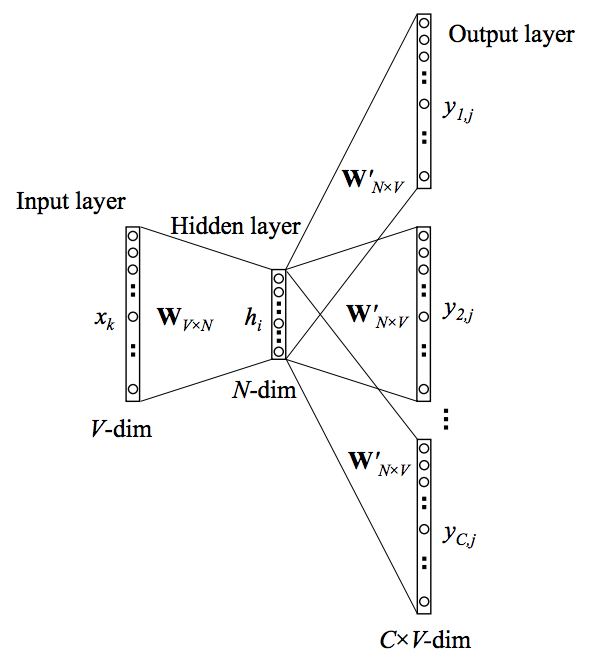
\includegraphics{images/skip_gram.png}
\caption{Réseau de neurones du modèle Skip-gram (source : Wikimedia).}
\label{skip_gram}
\end{center}
\end{figure}

Ce modèle a l'avantage de fournir de l'information syntaxique et sémantique sur les mots. En effet, des mots qui se retrouvent souvent dans des contextes similaires auront des vecteurs proches. Et s'ils se retrouvent dans les contextes similaires c'est qu'ils ont des fonctions grammaticales et des sens proches. Pour s'en apercevoir, nous avons projeté nos vecteurs dans $\mathbb{R}^{2}$ pour les visualiser en utilisant l'algorithme t-SNE \cite{van2008visualizing} qui préserve les voisinages (figure \ref{tsne_plot}).

\begin{figure}[h]
\begin{center}
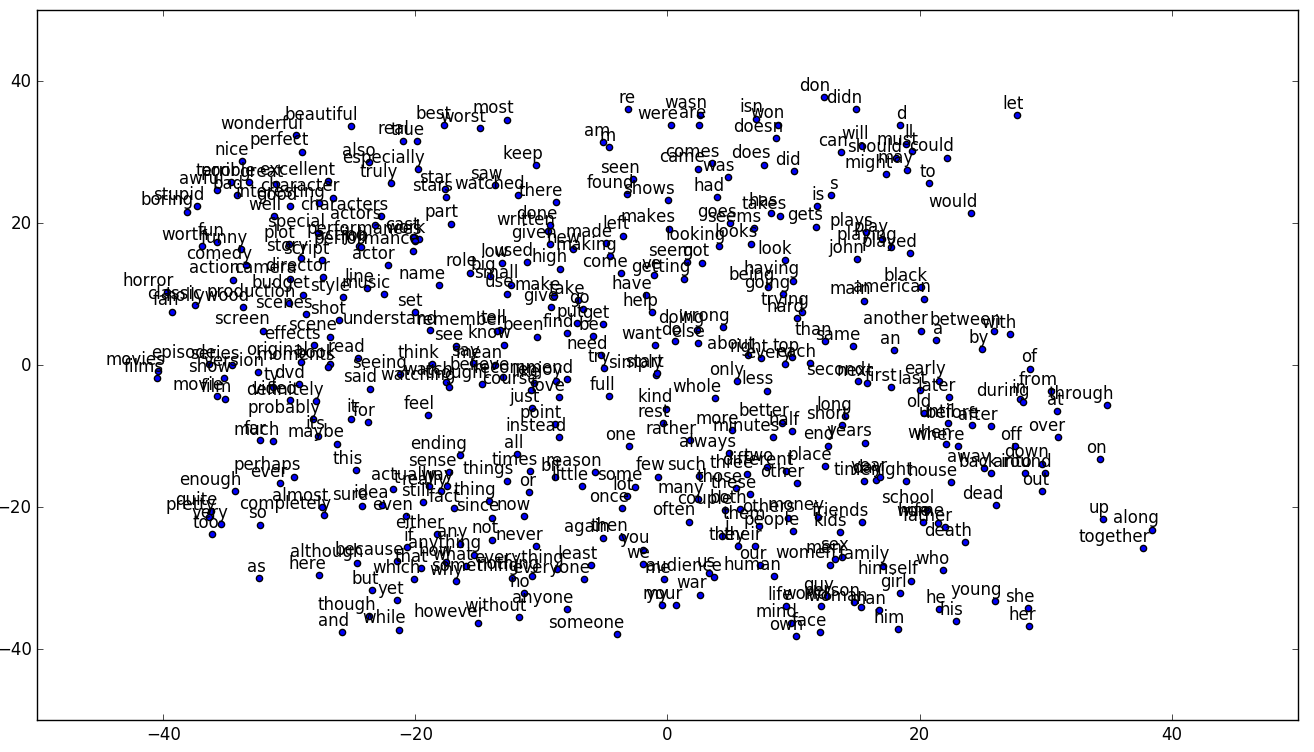
\includegraphics[scale=0.35]{images/tsne_plot.png}
\label{tsne_plot}
\end{center}
\end{figure}

En particulier, on peut remarquer la présence de clusters de mots. En particulier, nous avons mis en évidence dans la figure \ref{clusters} un cluster de mots liés au cinéma \ref{clusters} et un autre contenant des mots-outils.

\begin{figure}[h]
\begin{center}
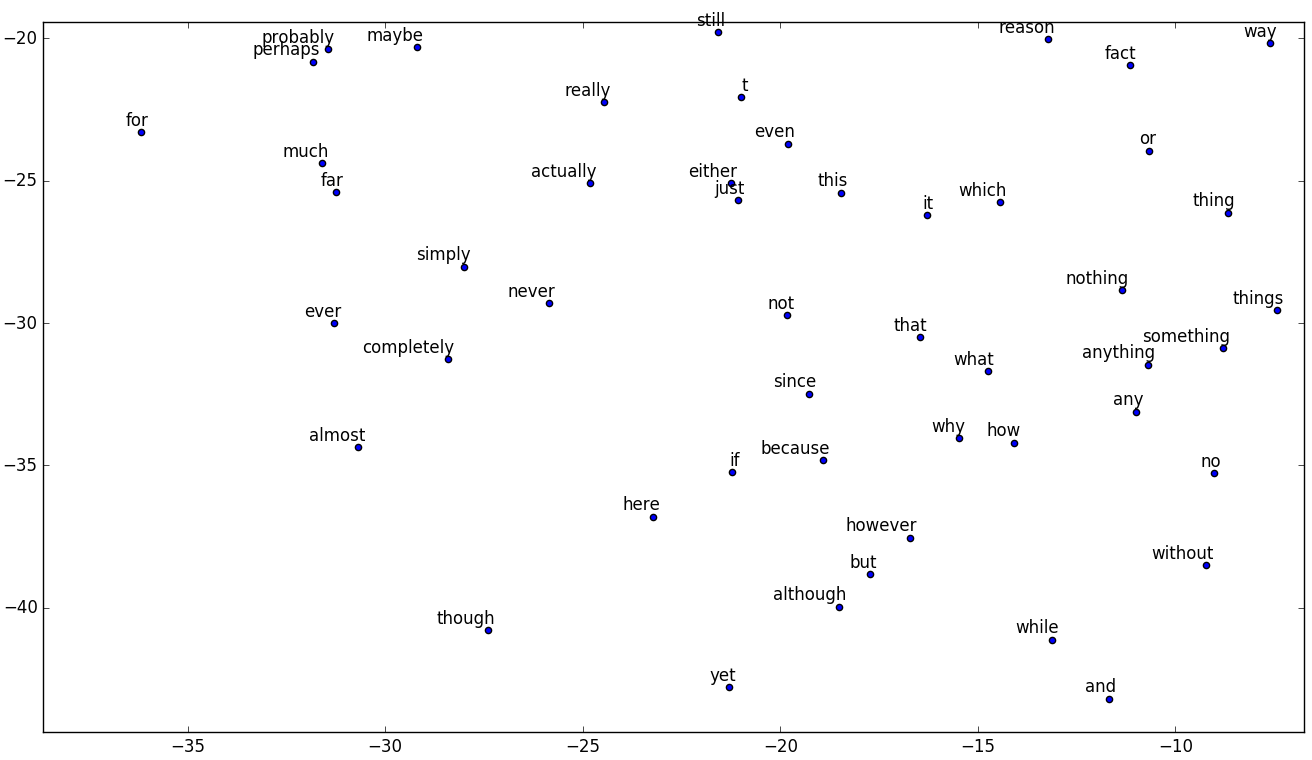
\includegraphics[scale=0.35]{images/cluster_cinema.png} \\
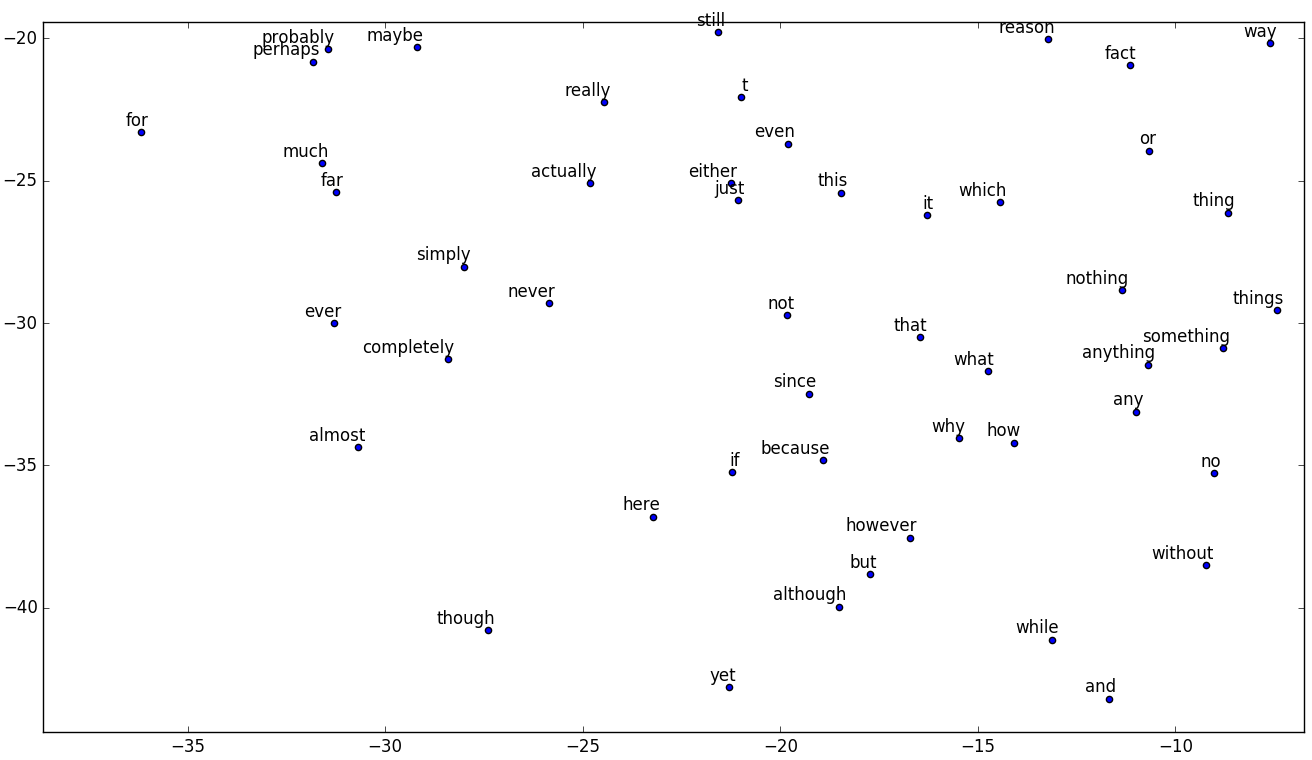
\includegraphics[scale=0.35]{images/cluster_toolwords.png}
\label{clusters}
\end{center}
\end{figure}

\subsubsection{Apprentissage}

Nous avons donc une représentation des mots cependant, nous avons besoin de représenter des textes. Une solution simple est de faire une combinaison linéaire des vecteurs représentants les mots du texte. Comme pour les sacs de mots, plusieurs variantes s'offrent à nous. Nous pouvons supposer que tous les mots ont un poids égal, l'application associant à un texte $t$ sont vecteur sera alors définie par :
$$
h_{vec}(t) = \frac{\sum_{w_{i} \in t}{tf_{i, t}v_{i}}}{\sum_{w_{i} \in t}{tf_{i, t}}} 
$$

Cependant, on peut aussi considérer que les mots ont des poids différents selon leur rareté, et donc comme pour les sacs de mots, nous allons pondérer par l'$IDF$ :
$$
h_{vec+idf}(t) = \frac{\sum_{w_{i} \in t}{tf_{i, t}idf_{i}v_{i}}}{\sum_{w_{i} \in t}{tf_{i, t}idf_{i}}}
$$

De même que pour les sacs de mots, nous avons mesurer la précision de la régression logistique et des forêts aléatoires avec comme entrées des vecteurs de mot. On retrouvera ces résultats dans la figure \ref{results_vec}.

\begin{figure}
\begin{center}
\begin{tabular}{|l|c|}
	\hline
	Forêt aléatoire à 100 estimateurs + Vect & 0.7954 \\
	\hline
	Forêt aléatoire à 100 estimateurs + Vect + TF-IDF & 0.79416 \\
	\hline
	Régression logistique + Vect & 0.81652 \\
	\hline
	Régression logistique + Vect + TF-IDF & 0.81688 \\
	\hline
\end{tabular}
\caption{Précisions des vecteurs de mot avec différents algorithmes (Vec : vecteurs de mots, TF-IDF : vecteurs de mot pondérés par IDF)}
\label{results_vec}
\end{center}
\end{figure}

Ici contrairement aux sacs de mots, la pondération des mots par l'$IDF$ n'offre aucune amélioration. Cela peut s'expliquer par le fait que des mots rares mais ne portant aucun sens utile pour l'analyse de sentiment vont diminuer l'importance d'autres mots importants pour l'analyse de sentiment mais plus courants. 

\subsection{Conclusion}

% Courbes d'apprentissage

% Il est possible de booster en faisant de l'apprentissage d'ensemble

% Il est nécessaire de prendre en compte l'ordre des mots

\section{Prise en compte de l'ordre des mots}

\section{Conclusion}

\bibliographystyle{plain}
\bibliography{sentiment_analysis}

\end{document}
